\documentclass[11pt, a4paper]{article}

\usepackage{amsmath}
\usepackage{amsfonts} %Matheschriften
\usepackage{amssymb} %Mathesymbole
%\usepackage{mathptmx} % Einstellung für Schriften und Sonderzeichen in mathematischen Umgebungen
                        % ändert SChriftfont
\usepackage{wasysym} % Stellt diverse Sonderzeichen bereit
\usepackage{siunitx}
\usepackage{float}
\usepackage{microtype}
\usepackage{graphicx}
\usepackage{hyperref}
\usepackage{xcolor}
\usepackage[section]{placeins}
% allows for temporary adjustment of side margins
\usepackage{changepage}
\usepackage{rotating}


\usepackage[ngerman]{babel}
\addto\captionsngerman{%
 \renewcommand{\abstractname}{Einleitung}}

\title{Versuch 1:Röntgenstrahlung}
\author{Team 4-11: Jascha Fricker, Benedict Brouwer}

\begin{document}
    \maketitle

    \tableofcontents

    \newpage

    \section{Einleitung}

    Röntgenstrahlen werden in vielen verschiedenen Bereichen benutzt. So z. B. als bildgebendes Verfahren in der Medizin oder in der zerstörungsfreien Prüfung von Werkstücken. In diesem Versuch werden die grundlegenden Eigenschaften von Röntgenstrahlen, sowie die Emissions und Absorbtionsfähigkeit von Materialien untersucht.

    \section{Theorie}

    \subsection{Röntgenstrahlung}

    Die Energie eines Photons kann durch die Wellenlänge mithilfe des plankschen Wirkungsquantums berechnet werden.
    \begin{align}
        E = \frac{h \cdot c}{\lambda}
    \end{align}
    In einer Röntgenröhre werden Röntgenstrahlen durch die Bremsstrahlung von durch ein elektrisches Feld beschleunigten Elektronen erzeugt. Die minimale Wellenlänge
    \begin{align}
        \lambda_{min} = \frac{h \cdot c}{E_{max}} &= \frac{h \cdot c}{e \cdot U} \\
        h &= \frac{\lambda_{min} e U}{c} \label{eq:plank}
    \end{align}
    ist durch die Beschleunigungsspannung $U$ bestimmt.

    \subsection{Beugung an Kristallgittern}

    Die Beugung an Kristallgittern wird durch die Bragg-Gleichung beschrieben.
    \begin{align}
        2 \cdot d \cdot \sin \theta = g \cdot sin \theta = n \lambda \\
        g = \frac{n \lambda}{sin \theta} \label{eq:gitter}
    \end{align}
    Hierbei ist $g$ die Gitterkonstante, $\theta$ der Beugungswinkel und $\lambda$ die Wellenlänge des in diesem Winkel reflektierten Röntgenstrahls. Mit diesem Effekt kann das Röntgenspektrum bestimmt werden.

    \subsection{Röntgenspektrum}

    Das Röntgenspektrum wird duch die Beschleunigungsspannnung und das Material der Röntgenröhre mit den charackteristischen Energieniveaus bestimmt. In diesem Versuch können die untersten zwei Energieniveaus, die $K_{\alpha}$ und $K_{\beta}$ Linien, erkannt werden.
    \subsection{Absorbtionsfähigkeit}

    Die Transmisson eines Materials
    \begin{align}
        T(\lambda) = \frac{I(\lambda)}{I_{0}(\lambda)} \label{eq:transmission}
    \end{align}
    wird als Quotient aus der Intensität des durch das Material durchgelassenen Röntgenstrahls und der Intensität des ungestörten Röntgenstrahls bestimmt. Die Absorbtionsfähigkeit eines Materials
    \begin{align}
        A(\lambda) = 1 - T(\lambda) = \frac{I_{0}(\lambda) - I(\lambda)}{I_{0}(\lambda)}
    \end{align}
    ist die Intensiät, die nicht transmittiert wird.

    \subsection{Totzeit}
    % Jascha hat eine Frage
    Das Geiger-Müller Zählrohr kann direkt nach einem Event für eine bestimmte Zeit nicht mehr zählen. Diese Zeit wird als Totzeit bezeichnet. Die Totzeit ist implizit abhängig vom Strom, der durch die Röntgenröhre fließt. Es gilt
    \begin{align}
        R_{z} = R \cdot e^{-R \cdot t} \circeq r \cdot I \cdot e^{-r \cdot \tau \cdot I}. \label{eq:totzeit}
    \end{align}

    \section{Ergebnisse}

    \subsection{Winkelunsicherheit}
    Durch die verschiebung der Messreihen untereinander kann die Genauigkeit der Winkel bestimmt werden. Der Unterschied der gemessenen Winkel wird als Unischerheit der Winkelmessung benutzt. Aus der Verschiebung der zwei Messreihen im Graph \ref{fig:wink} von etwa $0,1^{\circ}$ kann eine Unsicherheit von etwa $0,1^{\circ}$ geschätzt werden. So ergibt sich eine gesamte Winkelunsicherheit von $0,15^{\circ}$.

    \begin{figure}
        \centering
        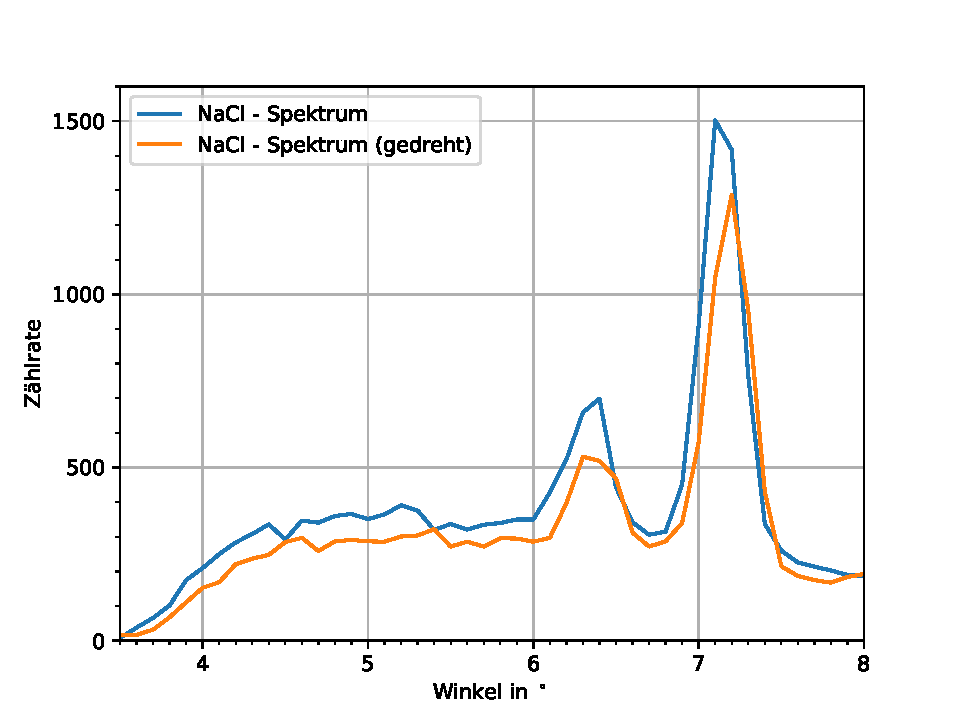
\includegraphics[width=0.8\textwidth]{Winkelfehler.pdf}
        \caption{Winkelfehler}
        \label{fig:wink}
    \end{figure}

    \subsection{Röntgenspektrum} \label{ront}

    Mithilfe der Drehkristallmethode konnte das Röntgenspektrum (Graph \ref{fig:roentgenspektrum}) gemessen werden. Aus diesem wurden die Maxima der $K_{\alpha}$ und $K_{\beta}$ Linien ersten, zweiten und dritten Grades bestimmt. Die gemessenen Werte sind in der Tabelle \ref{tab:roentgenspektrum} aufgeführt. Aus diesen konnten die endgültigen Ergebnisse für Wellenlänge und Enegie der $K_{\alpha}$ und $K_{\beta}$ Linien berechnet werden. Die Ergebnisse sind in der Tabelle \ref{tab:linienerg} aufgeführt.

    \begin{table}
        \centering
        \caption{Ergebnisse Emissionsspektrum}
        \label{tab:linienerg}
        \begin{tabular}{c|c|c}
            & $K_{\alpha}$ & $K_{\beta}$ \\
            \hline
            Wellenlänge $\lambda$ in pm & 70.79(57) & 62.79(38) \\
            Energie $E$ in keV & 17.545(93) & 19.75(12) \\
            Literaturwert Energie \cite{lin} in keV & 17,47934 & 19,6083
        \end{tabular}
    \end{table}

    \begin{table}[h]
        \centering
        
        \begin{tabular}{c|c|c|c} \label{tab:roentgenspektrum}
        & \textbf{$n = 1$} & \textbf{$n = 2$} & \textbf{$n = 3$} \\ 
        \hline
        Winkel $K_{\alpha}$ in Grad & 7.15(15) & 14.50(15) & 22.10(15)\\ 
        Winkel $K_{\beta}$ in Grad & 6.40(15) & 12.80(15) & 19.55(15)\\ 
        Wellenlänge $K_{\alpha}$ in pm & 70.2(15) & 70.61(72) & 70.73(46) \\ 
        Wellenlänge $K_{\beta}$ in pm & 62.9(15) & 62.48(72) & 62.91(47)\\ 
        Energie $K_{\alpha}$ in keV & 17.66(37) & 17.56(18) & 17.53(12)\\ 
        Energie $K_{\beta}$ in keV & 19.72(47) & 19.84(23) & 19.71(15)\\ 
        \end{tabular}
        \caption{Messwerte Emissionsspektrum}
    \end{table}

    \begin{figure}
        \centering
        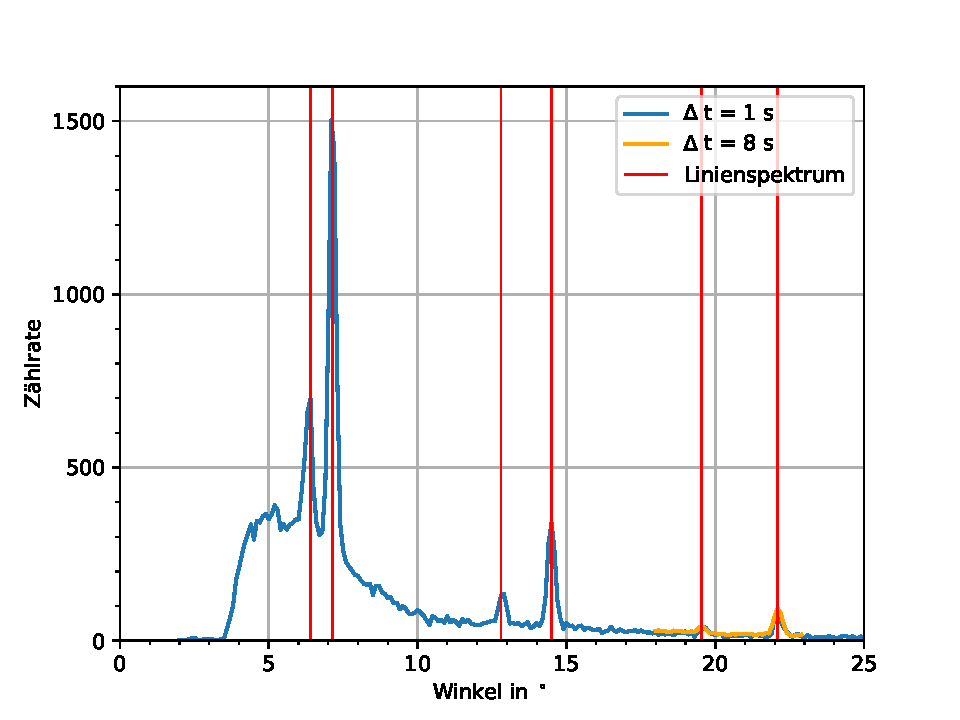
\includegraphics[width=0.8\textwidth]{NaCl-Spektrum.pdf}
        \caption{Röntgenspektrum}
        \label{fig:roentgenspektrum}
    \end{figure}

    \subsection{Absorbtionsfähigkeit}

    Aus dem Emissionsspektrum ohne Zirkonium-Folie und aus dem mit Zirkoniumfolie kann die Wellenlängenabhängige Transmission mit Gleichung (\ref{eq:transmission}) berechnet und in Plot \ref{fig:trans} geplottet werden. In diesem Plot erkennt man Absorbtionskante und deren Eigenschaften
    \begin{align}
        \text{Wellenlänge} \ \ \lambda &= 67,7(13) \si{\pico\meter}\\
        \text{Energie} \ \ E &= 18.31(35) \text{keV}.
    \end{align}

    \begin{figure}
        \centering
        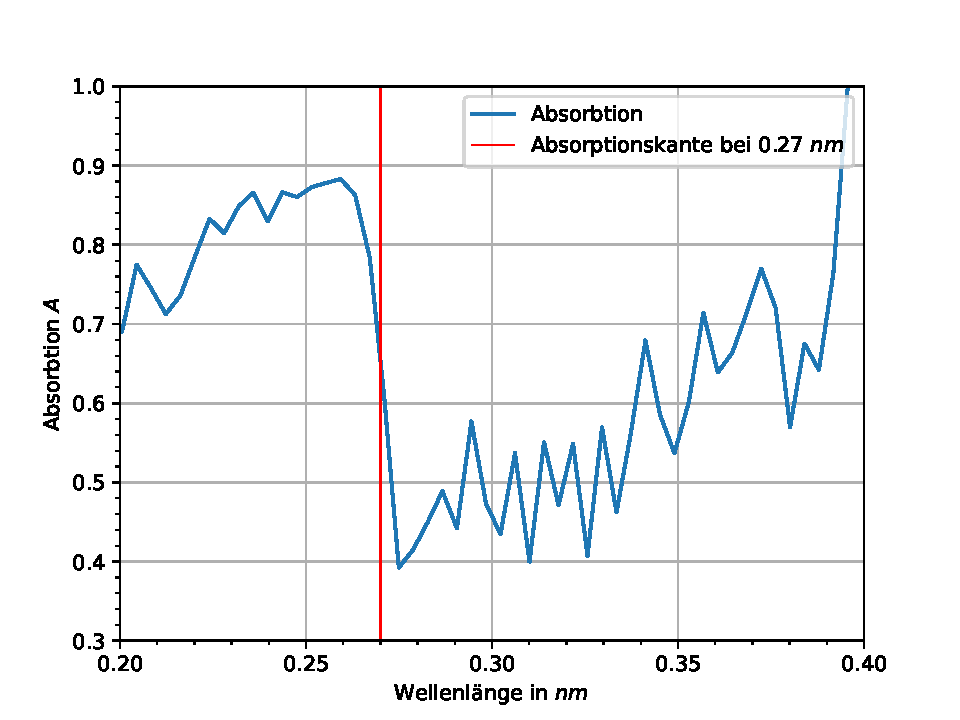
\includegraphics[width=0.8\textwidth]{Zirkonium.pdf}
        \caption{Absorbtion}
        \label{fig:trans}
    \end{figure}

    \subsection{LiF-Kristall}
    Durch die Mittelwerte der zwei gemessen Winkelordnungen mit den Werten
    \begin{align}
        K_{\alpha} &= 10.053(84) \si{\degree} \\
        K_{\beta} &= 8.903(84) \si{\degree}
    \end{align}
    der Linien im Röntgenspektrum des LiF Kristall (Siehe \ref{fig:LiF}) und die in \ref{ront} berechneten Wellenlängen der Linien kann mit Formel \ref{eq:gitter} die Gitterkonstante
    \begin{align}
        g_{LiF} = 404,7(38) \si{\pico\meter} \\
        \text{Theoriewert \cite{lif} } 402,6 \si{\pico\meter}
    \end{align}
    des LiF-Kristalls bestimmt werden.

    \begin{figure}
        \centering
        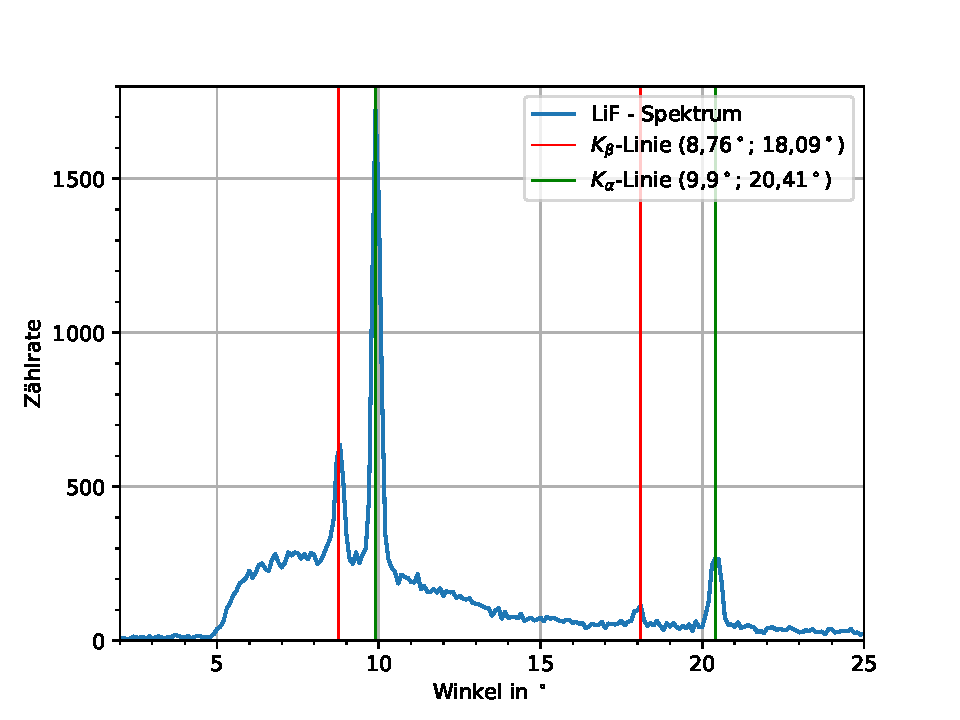
\includegraphics[width=0.8\textwidth]{LiF-Spektrum.pdf}
        \caption{Röntgenspektrum LiF Kristall}
        \label{fig:LiF}
    \end{figure}

    \subsection{Detektor-Totzeit}
    Durch die Zählrate der $K_{\alpha}$ Linie bei verschienen Strömen und einen Fit der Formel \ref{eq:totzeit}, welches im Graph \ref{fig:totzeit} dargestellt ist, konnte die Detektor-Totzeit
    \begin{align}
        \tau = 94,5(80) \si{\micro\second}
    \end{align}
    bestimmt werden. Die Rohdaten sind im Anhang \ref{fig:totzeitroh} zu finden.

    \begin{figure}
        \centering
        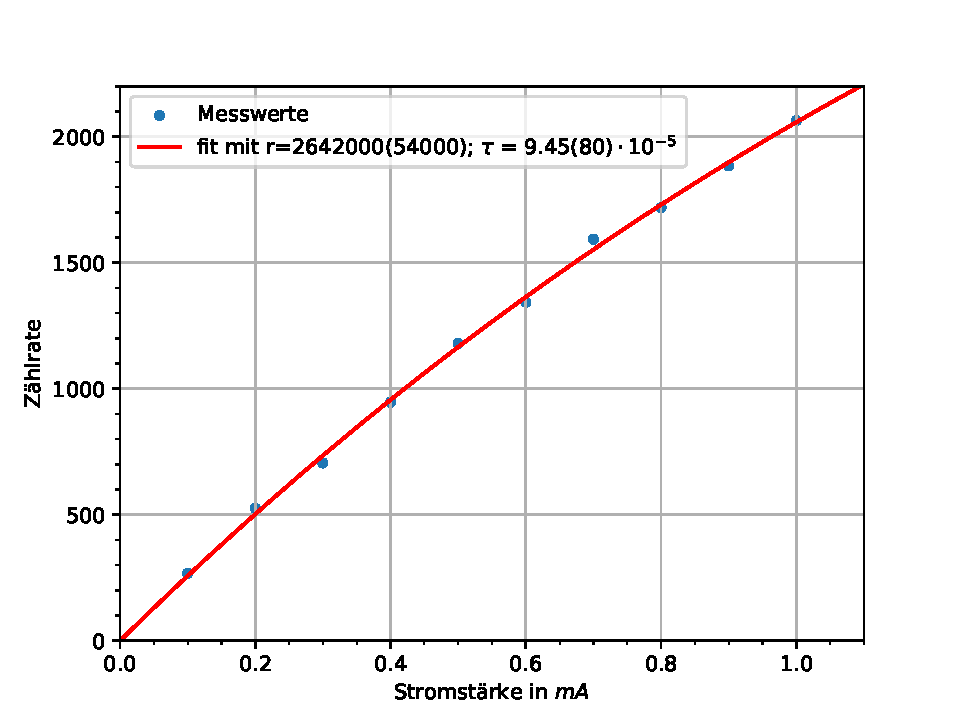
\includegraphics[width=0.8\textwidth]{Detektortotzeit.pdf}
        \caption{Detektor-Totzeit}
        \label{fig:totzeit}
    \end{figure}

    \subsection{Planksches Wirkungsquantum}

    Durch die Extrapolation der Grenzwellenlänge $\lambda_0$ bei verschiedenen Strömen aus dem linearen Bereich des Emissionsspektrums, wie im Graph \ref{fig:plank} dargestellt, kann das Planksche Wirkungsquantum
    \begin{align}
        h = 9.2(15) \cdot 10^{-34} \text{Js} \\
        \text{Theoriewert \cite{plank}} \ \  h = 6,6260755(40) \cdot 10^{34} \text{Js}
    \end{align}
    mithilfe der Formel \ref{eq:plank} bestimmt werden. Als Ableseungenauigkeit der Grenzwellenlänge wurden $2$ pm angenommen.

    \begin{figure}
        \centering
        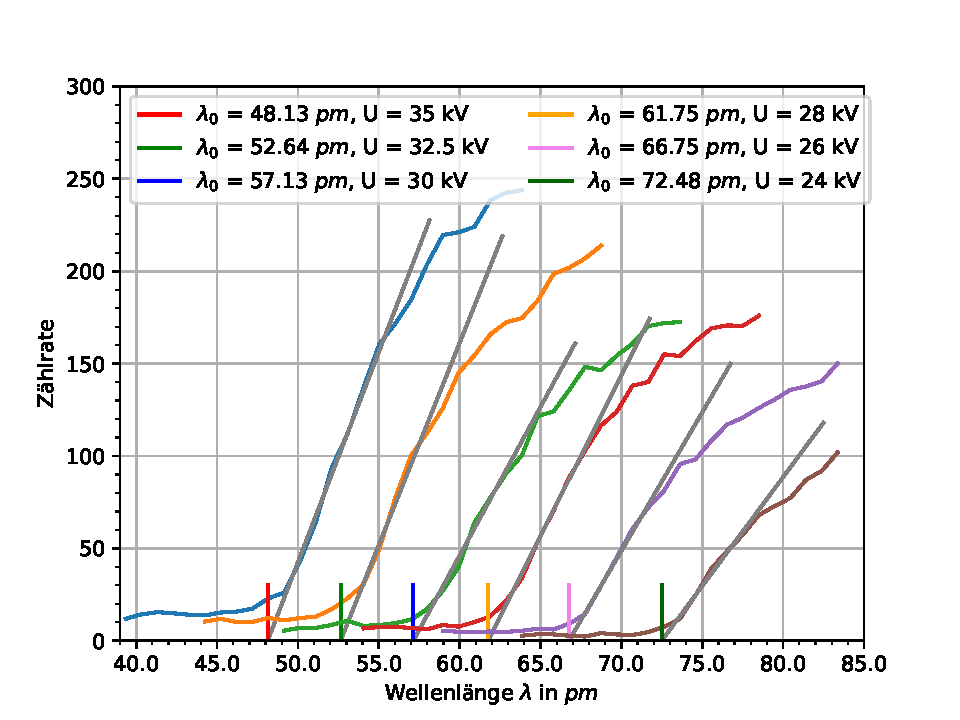
\includegraphics[width=0.8\textwidth]{Plank.pdf}
        \caption{Planksches Wirkungsquantum}
        \label{fig:plank}
    \end{figure}

    \section{Diskussion}

    Bei dem meisten Messungen kann der gemessene Wert mit dem Theoriewert verglichen werden. Bei den $K_{\alpha}$ und $K_{\beta}$ Linien und der Gitterkonstanten liegen diese auch im Konfidenzintervall der Messungen. Nur bei der Berechnung der Plankschen Winrkungsquantums liegt ein doch erheblicher Fehler vor.  Zwar liegt der Wert in der richtigen Größenordnung, er weicht aber erheblich vom Literaturwert ab, wir wissen nicht woran das liegt, (Wurde im Kolloquium besprochen)  aber es könnte zum einen an einer Abweichung des Messwert der Spannung liegen. Dieser wurde nur bei dem letzten Versuch verwendet. Für die weiteren Messwerte wurden keine Theoriewerte gefunden, die Unicherheiten liegen jedoch im erwarteten Bereich.

    \section{Anhang}

    \subsection{Detektortotzeit}

    \begin{figure}
        \centering
        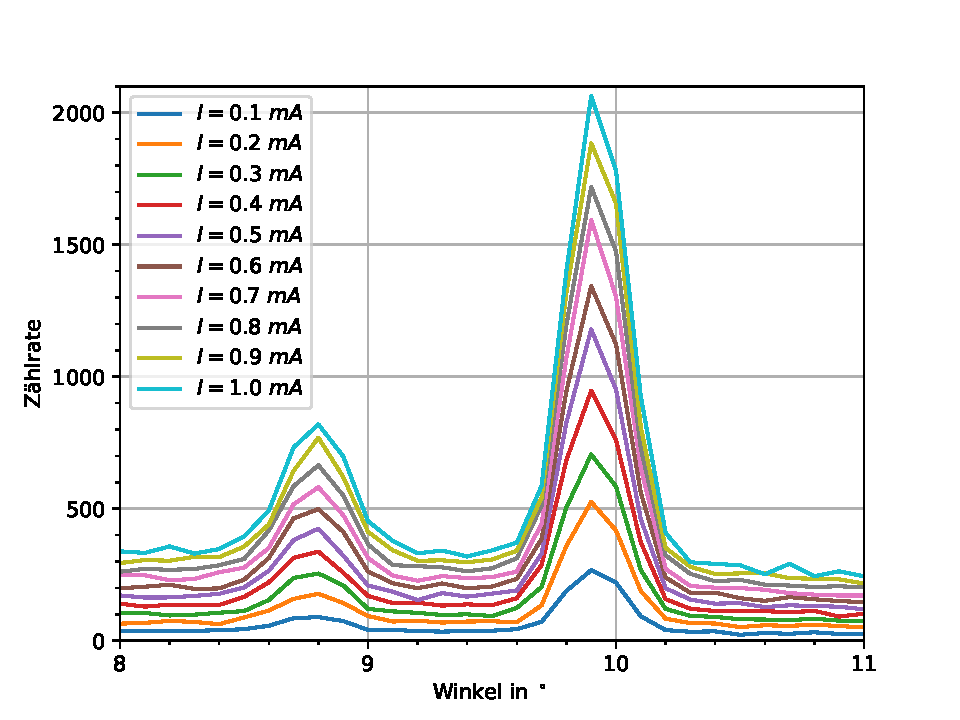
\includegraphics[width=0.8\textwidth]{DetektortotzeitRoh.pdf}
        \caption{Detektor-Totzeit Rohdaten}
        \label{fig:totzeitroh}
    \end{figure}


    \bibliographystyle{plain}
    \bibliography{literature}

\end{document}